% 
% exemplo genérico de uso da classe iiufrgs.cls
% $Id: iiufrgs.tex,v 1.1.1.1 2005/01/18 23:54:42 avila Exp $
% 
% This is an example file and is hereby explicitly put in the
% public domain.
% 
\documentclass[cic,tc]{iiufrgs}
% Para usar o modelo, deve-se informar o programa e o tipo de documento.
% Programas :
% * cic       -- Graduação em Ciência da Computação
% * ecp       -- Graduação em Ciência da Computação
% * ppgc      -- Programa de Pós Graduação em Computação
% * pgmigro   -- Programa de Pós Graduação em Microeletrônica
% 
% Tipos de Documento:
% * tc                -- Trabalhos de Conclusão (apenas cic e ecp)
% * diss ou mestrado  -- Dissertações de Mestrado (ppgc e pgmicro)
% * tese ou doutorado -- Teses de Doutorado (ppgc e pgmicro)
% * ti                -- Trabalho Individual (ppgc e pgmicro)
% 
% Outras Opções:
% * english    -- para textos em inglês
% * openright  -- Força início de capítulos em páginas ímpares (padrão da
% biblioteca)
% * oneside    -- Desliga frente-e-verso
% * nominatalocal -- Lê os dados da nominata do arquivo nominatalocal.def

% === PACKAGES ===
% Use unicode
\usepackage[utf8]{inputenc}   % pacote para acentuação
% Necessário para incluir figuras
\usepackage{graphicx}         % pacote para importar figuras
\usepackage{times}            % pacote para usar fonte Adobe Times
% \usepackage{palatino}
% \usepackage{mathptmx}       % p/ usar fonte Adobe Times nas fórmulas
\usepackage[alf,abnt-emphasize=bf, abnt-etal-list=0, abnt-etal-cite=2]{abntex2cite}	% pacote para usar citações abnt
\usepackage{verbatim}
\usepackage{amsmath}
\usepackage{algorithm}
\usepackage[noend]{algpseudocode}
\usepackage{color, colortbl}
\usepackage{placeins}
\usepackage{chngpage}
\usepackage{hyperref}
\usepackage{rotating}
\usepackage{graphics}
\usepackage{array}

% === DEFINITIONS === 
\floatname{algorithm}{Algoritmo}
\graphicspath{ {./figuras/} }
\renewcommand{\arraystretch}{1.5}
\definecolor{darkorange}{rgb}{0.9647058823529412, 0.6980392156862745, 0.4196078431372549}
\definecolor{lightorange}{rgb}{0.9768, 0.79608, 0.61176}
\newcolumntype{o}{>{\columncolor{lightorange}}r}
\newcolumntype{P}[1]{>{\centering\arraybackslash}p{#1}}

% comandos miraculosos para evitar quebra de palavras
\tolerance=1
\emergencystretch=\maxdimen
\hyphenpenalty=10000
\hbadness=10000


% 
% Informações gerais
% 
\title{Portal de Vagas - implementação de uma ferramenta para divulgação de bolsas e estágios a alunos}

\author{Flesch}{Jean Ampos}
% alguns documentos podem ter varios autores:
% \author{Flaumann}{Frida Gutenberg}
% \author{Flaumann}{Klaus Gutenberg}

% orientador e co-orientador são opcionais (não diga isso pra eles :))

\advisor[Profa.~Dra.]{Galante}{Renata}
% \coadvisor[Prof.~Dr.]{Knuth}{Donald Ervin}

% a data deve ser a da defesa; se nao especificada, são gerados
% mes e ano correntes
% \date{maio}{2001}

% o local de realização do trabalho pode ser especificado (ex. para TCs)
% com o comando \location:
% \location{Itaquaquecetuba}{SP}

% itens individuais da nominata podem ser redefinidos com os comandos
% abaixo:
% \renewcommand{\nominataReit}{Prof\textsuperscript{a}.~Wrana Maria Panizzi}
% \renewcommand{\nominataReitname}{Reitora}
% \renewcommand{\nominataPRE}{Prof.~Jos{\'e} Carlos Ferraz Hennemann}
% \renewcommand{\nominataPREname}{Pró-Reitor de Graduação}
\renewcommand{\nominataPRAPG}{Prof.~Vladimir Pinheiro do Nascimento}
\renewcommand{\nominataPRAPGname}{Pró-Reitor de Graduação}
% \renewcommand{\nominataDir}{Prof.~Philippe Olivier Alexandre Navaux}
% \renewcommand{\nominataDirname}{Diretor do Instituto de Inform{\'a}tica}
\renewcommand{\nominataCoord}{Prof.~Sérgio Luis Cechin}
\renewcommand{\nominataCoordname}{Coordenador do Curso de Ciência de Computação}
% \renewcommand{\nominataBibchefe}{Beatriz Regina Bastos Haro}
% \renewcommand{\nominataBibchefename}{Bibliotec{\'a}ria-chefe do Instituto de Inform{\'a}tica}
% \renewcommand{\nominataChefeINA}{Prof.~Jos{\'e} Valdeni de Lima}
% \renewcommand{\nominataChefeINAname}{Chefe do \deptINA}
% \renewcommand{\nominataChefeINT}{Prof.~Leila Ribeiro}
% \renewcommand{\nominataChefeINTname}{Chefe do \deptINT}

% A seguir são apresentados comandos específicos para alguns
% tipos de documentos.

% Relatório de Pesquisa [rp]:
% \rp{123}             % numero do rp
% \financ{CNPq, CAPES} % orgaos financiadores

% Trabalho Individual [ti]:
% \ti{123}     % numero do TI
% \ti[II]{456} % no caso de ser o segundo TI

% Monografias de Especialização [espec]:
% \espec{Redes e Sistemas Distribuídos}      % nome do curso
% \coord[Profa.~Dra.]{Weber}{Taisy da Silva} % coordenador do curso
% \dept{INA}                                 % departamento relacionado

% 
% palavras-chave
% iniciar todas com letras minúsculas, exceto no caso de abreviaturas
% 
\keyword{Rede social}
\keyword{Aplicação web}
\keyword{Experiência profissional}
\keyword{\textit{User Experience}}
%\keyword{\textit{Networking}}

%\settowidth{\seclen}{1.10~}

% 
% inicio do documento
% 
\begin{document}

% folha de rosto
% às vezes é necessário redefinir algum comando logo antes de produzir
% a folha de rosto:
% \renewcommand{\coordname}{Coordenadora do Curso}
\maketitle

% dedicatoria
%\clearpage
%\begin{flushright}
%     \mbox{}\vfill
%     {\sffamily\itshape
%       ``If I have seen farther than others,\\
%       it is because I stood on the shoulders of giants.''\\}
%     --- \textsc{Sir~Isaac Newton}
%\end{flushright}

% agradecimentos
\chapter*{Agradecimentos}
~meus agradecimentos vão aqui~



% resumo na língua do documento
\begin{abstract}
	É durante a graduação que geralmente ocorrem as primeiras experiências profissionais dos alunos, sejam elas provenientes de bolsas ofertadas pela própria universidade ou de estágios em empresas do mercado de trabalho. Para ajudar na divulgação de vagas em ambas as modalidades, a UFRGS disponibiliza ferramentas de acesso à informação aos seus discentes como o e-mail de graduação e o site do Mural de Bolsas.
    
    Este  trabalho  objetiva realizar  uma  releitura  do atual Mural  de  Bolsas, desenvolvendo  uma rede social que aproxime ainda mais alunos e professores, possibilite interações mais dinâmicas e forneça um canal de comunicação para os usuários, tudo isto centralizado em uma única ferramenta. Desta forma, é possível desenvolver soluções mais eficientes e precisas no gerenciamento das vagas ofertadas, utilizando pesquisas mais refinadas e complexas como as baseadas no desempenho acadêmico do aluno, por exemplo.
    
    Acredita-se que a rede social contribuirá para uma maior organização nas divulgação de bolsas e estágios na universidade e um consequente ingresso mais qualificado de alunos, privilegiando àqueles com real interesse nas vagas e melhor desempenho em seu curso de graduação.
    \newline
%\textit{framework}
%\cite{MasterMichaels2014}
\end{abstract}

% resumo na outra língua
% como parametros devem ser passados o titulo e as palavras-chave
% na outra língua, separadas por vírgulas
\begin{englishabstract}{
Portal de Vagas - implementation of a tool to promote scholarships and internships to students}{Social network.  Web application. Professional experience. User Experience}
	It is during the graduation that usually the first professional experiences of the students occur, whether they come from scholarships offered by the university itself or from internships in companies of the labor market. To help publicize vacancies in both modalities, UFRGS provides tools for accessing information to its students, such as the graduation e-mail and the Bolsa Mural website.
    
    This work aims to re-read the current Mural of Scholarships, developing a social network that brings even more students and teachers, enables more dynamic interactions and provides a channel of communication for users, all centralized in a single tool. In this way, it is possible to develop more efficient and precise solutions in the management of offered vacancies, using more refined and complex researches such as those based on the academic performance of the student, for example.

    It is believed that the social network will contribute to a greater organization in the dissemination of scholarships and internships in the university and a consequent more qualified admission of students, privileging those with real interest in the vacancies and better performance in its undergraduate course.

\end{englishabstract}

% lista de figuras
\listoffigures

% lista de tabelas
\listoftables

% lista de abreviaturas e siglas
% o parametro deve ser a abreviatura mais longa
\begin{listofabbrv}{UFRGS}
    \item[HTML] \textit{Hyper Text Markup Language}
    \item[CSS] \textit{Cascading Style Sheets}
    \item[PHP] \textit{PHP: Hypertext Preprocessor}
    \item[JS] \textit{JavaScript}
    \item[SQL] \textit{Structured Query Language}
    \item[MVC] \textit{Model-view-controller}
    \item[MB] Mural de Bolsas
    \item[UFRGS] Universidade Federal do Rio Grande do Sul
    \item[SGBD] Sistema de Gerenciamento de Banco de dados
    \item[XAMPP] \textit{X - Apache - MySQL - PHP - Perl}
\end{listofabbrv}

% idem para a lista de símbolos
% \begin{listofsymbols}{$\alpha\beta\pi\omega$}
%     \item[$\sum{\frac{a}{b}}$] Somatório do produtório
%     \item[$\alpha\beta\pi\omega$] Fator de inconstância do resultado
% \end{listofsymbols}

% sumario
\tableofcontents

% ========== CAP 1 ==============
\chapter{Introdução}

Texto introdução

% ========== CAP 2 ==============
\chapter{Levantamento Bibliográfico}

Texto cap 2

% ========== CAP 3 ==============
\chapter{Metodologia de desenvolvimento}
\label{metodologiaDesenvolvimento}
Este capítulo apresenta a proposta e implementação de um protótipo de rede social para criação e divulgação de vagas em bolsas na universidade e estágios. Inicialmente é realizado um levantamento de requisitos da aplicação. Em seguida, são detalhados a arquitetura e o projeto de banco de dados utilizados como guias para o desenvolvimento da rede social. Na sequência, o processo de implementação do sistema é detalhado, exibindo tomadas de decisões baseadas em padrões de projeto em engenharia de software.

\section{Visão Geral}
O objetivo da rede social é apresentar de uma maneira mais centralizada, interativa, intuitiva e organizada listas de vagas disponíveis tanto em bolsas na universidade quanto em estágios dentro e fora do meio acadêmico. Com a centralização de informações, os usuários poderiam através do seu login do INF pesquisar, recomendar e candidatar-se a vagas ofertadas e dados pessoais, profissionais ou acadêmicos, como histórico escolar, solicitados na vaga já seriam encaminhados automaticamente. Ainda, por ser uma rede social, é possível explorar uma maior interação entre os usuários, promovendo um networking e facilitando indicações a vagas futuras.

O ambiente implementado é um protótipo de aplicação Web baseado em uma arquitetura centralizada em dados \cite{pressman}, uma vez que é o padrão mais utilizado na Internet \cite{kurose}. A rede social pode ser acessada por navegadores Web mais modernos que possuem suporte às tecnologias HTML5 e CSS3. Em especial, todos os navegadores mais utilizados atualmente como Google Chrome, Mozilla Firefox, Opera, Safari e Edge.

O desenvolvimento no lado servidor foi realizado utilizando o motor de template Twig para a linguagem PHP, pois fornece recursos que facilitam a implementação de uma arquitetura MVC, além de possuir uma sintaxe que aumenta a legibilidade do código, facilitando sua manutenção. Complementarmente, para a comunicação com o banco de dados, foi utilizado um modelo Entidade-Relacionamento e o banco de dados escolhido foi SGBD relacional MySQL por ser uma ferramenta livre, popular e robusta\cite{mysql}.

O lado do cliente, por sua vez, foi constituído da união das tecnologias HTML5, CSS3, JavaScript e o framework jQuery. Este último é uma biblioteca de funções do JavaScript nativo que facilitam a prototipagem de aplicações e concedem suporte a diferentes tipos de browser, aumentando assim a portabilidade do sistema.


\section{Requisitos}
\label{metodologiaRequisitos}
Os requisitos de um sistema são descrições dos serviços fornecidos pelo sistema e suas restrições operacionais. Esses requisitos refletem as necessidades dos clientes de um sistema que ajuda a resolver a algum problema \cite{sommerville}. Frequentemente os requisitos de software são classificados em requisitos funcionais, que declaram os serviços que o sistema deve oferecer; e requisitos não funcionais, que são as restrições nas funções oferecidas pelo sistema. 

\subsection{Requisitos funcionais}
\label{requisitosRF}
Os requisitos funcionais referem-se sobre o que o sistema deve fornecer, ou seja, suas funções e informações. Preocupam-se com as funcionalidades, serviços e em como o sistema deve reagir em determinadas situações de acordo com entradas recebidas para satisfazer os requisitos do negócio. Abaixo, são listados os requisitos funcionais deste projeto:  

\begin{itemize}
    \item \textbf{RF01:} Para acessar o sistema, o usuário deverá efetuar o processo de login, utilizando um usuário e uma senha.
    
    \item \textbf{RF02:} O sistema deve permitir consultas sobre o banco de usuários, combinando zero ou mais filtros pré-definidos.
    
    \item \textbf{RF03:} O sistema deve permitir consultas sobre o banco de vagas, combinando zero ou mais filtros pré-definidos.
    
    \item \textbf{RF04:} O sistema deve permitir a inserção de novas vagas.
    
    \item \textbf{RF05:} O sistema deve permitir a edição de vagas existentes.
    
    \item \textbf{RF06:} O sistema deve permitir a exclusão lógica de vagas existentes.
    
    \item \textbf{RF07:} O sistema deve permitir a configuração de dados do usuário de acordo com sua preferência.
    
    \item \textbf{RF08:} O sistema deve permitir que um usuário siga ou deixe de seguir outros usuários unilateralmente.
    
    \item \textbf{RF09:} O sistema deve permitir que um usuário bloqueie ou desbloqueie outros usuários unilateralmente.
    
    \item \textbf{RF10:} O sistema deve permitir a inserção de novas postagens.
    
    \item \textbf{RF11:} O sistema deve permitir a edição de uma postagem já existente.
    
    \item \textbf{RF12:} O sistema deve permitir a exclusão lógica de uma postagem já existente.
    
    \item \textbf{RF13:} O sistema deve permitir que um usuário curta ou descurta uma postagem de outro usuário. 
    
    \item \textbf{RF14:} O sistema deve permitir que um usuário recomende outro usuário ou uma vaga.
\end{itemize}

\subsection{Requisitos não funcionais}
\label{requisitosRNF}
Os requisitos não-funcionais são restrições sobre os serviços ou as funções oferecidas pelo sistema. Elas incluem restrições de \textit{timing}, restrições sobre o processo de desenvolvimento e padrões. Os requisitos funcionais aplicam-se, frequentemente, ao sistema como um todo \cite{sommerville}. Em geral não se aplicam às características ou serviços individuais de sistema. Abaixo, são listados os requisitos não funcionais deste projeto:  

\begin{itemize}
    \item \textbf{RNF01:} O sistema deve ser hospedado em um servidor web.

    \item \textbf{RNF02:} Os dados deverão estar armazenados em um banco de dados relacional e centralizado.  

    \item \textbf{RNF03:} O sistema deve ser de fácil utilização.  

    \item \textbf{RNF04:} O sistema deve funcionar corretamente nos principais navegadores web.

    \item \textbf{RNF05:} O sistema deve ter um visual responsivo, possibilitando o uso em aparelhos mobile.

    \item \textbf{RNF06:} O sistema deve possibilitar dois tipos de usuários para acesso à ferramenta: usuários administradores, que terão acesso a todos os módulos do sistema; e usuários comuns, que poderão apenas consultar e recomendar vagas e interagir de maneira limitada com outros usuários.
\end{itemize}

\section{Arquitetura do sistema}
\label{arquiteturaSistema}
O desenvolvimento da rede social foi projetado para ser uma aplicação na web. Foram escolhidas duas arquiteturas diferentes: uma para centralizada em dados para atender às requisições de serviços do lado do servidor; e outra MVC, utilizada para a implementação da lógica e das telas da plataforma.

\subsection{Arquitetura centralizada em dados}
\label{arquiteturaCentralizadaDados}
A figura \ref{dataCenteredArchitecture} ilustra a arquitetura implementada. O ambiente do servidor, por residir em uma aplicação web receberá várias solicitações de usuários ao passo que ocorrem diversas interações no sistema \cite{kurose}, foi adotada uma configuração cliente-servidor (PRESSMAN) onde o banco de dados é centralizado no servidor que hospeda a rede social.

A linguagem de programação utilizada no desenvolvimento desta arquitetura foi o PHP. Esta é amplamente utilizada em páginas da Internet\footnote{\url{https://w3techs.com/technologies/overview/programming_language/all} Acesso em outubro de 2018}~e, mesmo com o advento de tecnologias emergentes como Node.js\footnote{\url{https://insights.stackoverflow.com/survey/2016\#technology} Acesso em outubro de 2018}~, mantém-se firme no mercado especialmente em questões \textit{server-side}. Por ser uma linguagem de código aberto, apresenta uma grande e participativa comunidade que constantemente desenvolve \textit{plugins}, \textit{frameworks} e bibliotecas para atender diversas demandas de desenvolvedores \cite{phpPatternsArticle2016}

\begin{figure}[ht]
    \caption{Arquitetura centralizada em dados.}
       	\begin{center}
            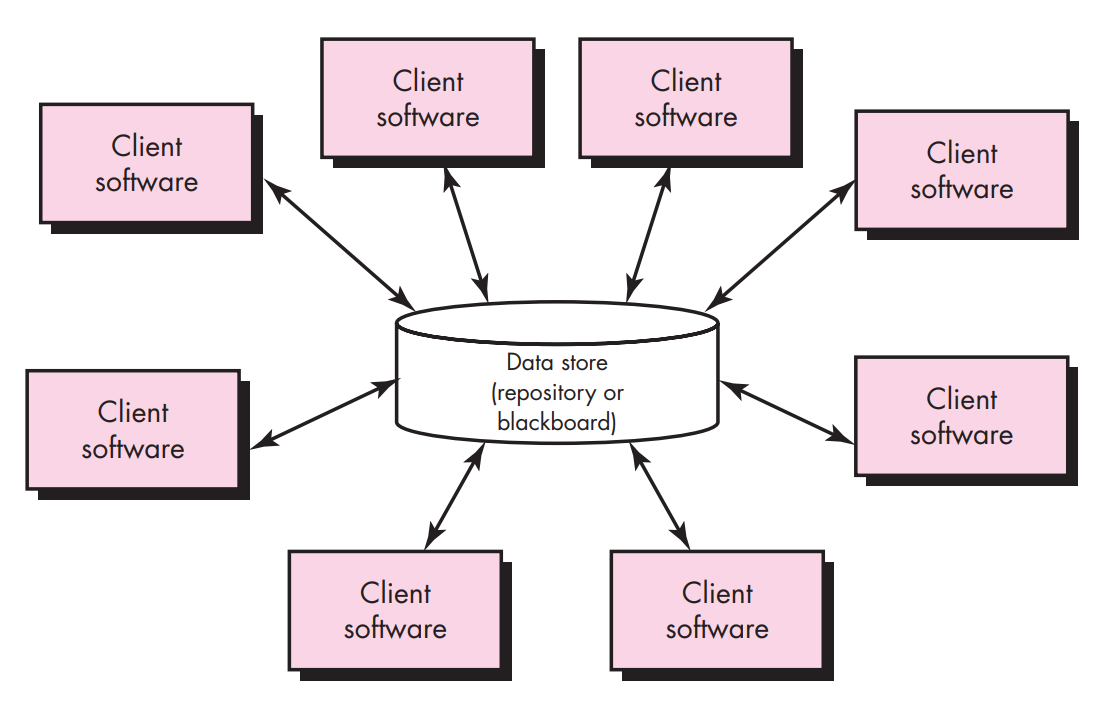
\includegraphics[width=0.68\textwidth]{arquitetura-centralizada-dados.png}
        \end{center}
    \label{dataCenteredArchitecture}
    \legend{Fonte: \cite{pressman}}
\end{figure}

\subsection{Arquitetura MVC}
\label{arquiteturaMVC}

Outra arquitetura de desenvolvimento de software adotada foi o MVC. Esta arquitetura desacopla a lógica da aplicação da interface do usuário, permitindo desenvolver, analisar e testar separadamente cada parte. O modelo engloba todo domínio específico à aplicação e seu processamento lógico como funcionalidades e acesso a dados externos e fontes de informação. A visão é responsável por exibir, na saída de dados, o conteúdo do modelo em um formato legível e requisitado pelo usuário final. O controlador coordena a comunicação entre o modelo e a visão de acordo com as requisições do usuário. A figura \ref{dataMVCArchitecture} ilustra a arquitetura implementada

\begin{figure}[ht]
    \caption{Arquitetura MVC.}
       	\begin{center}
            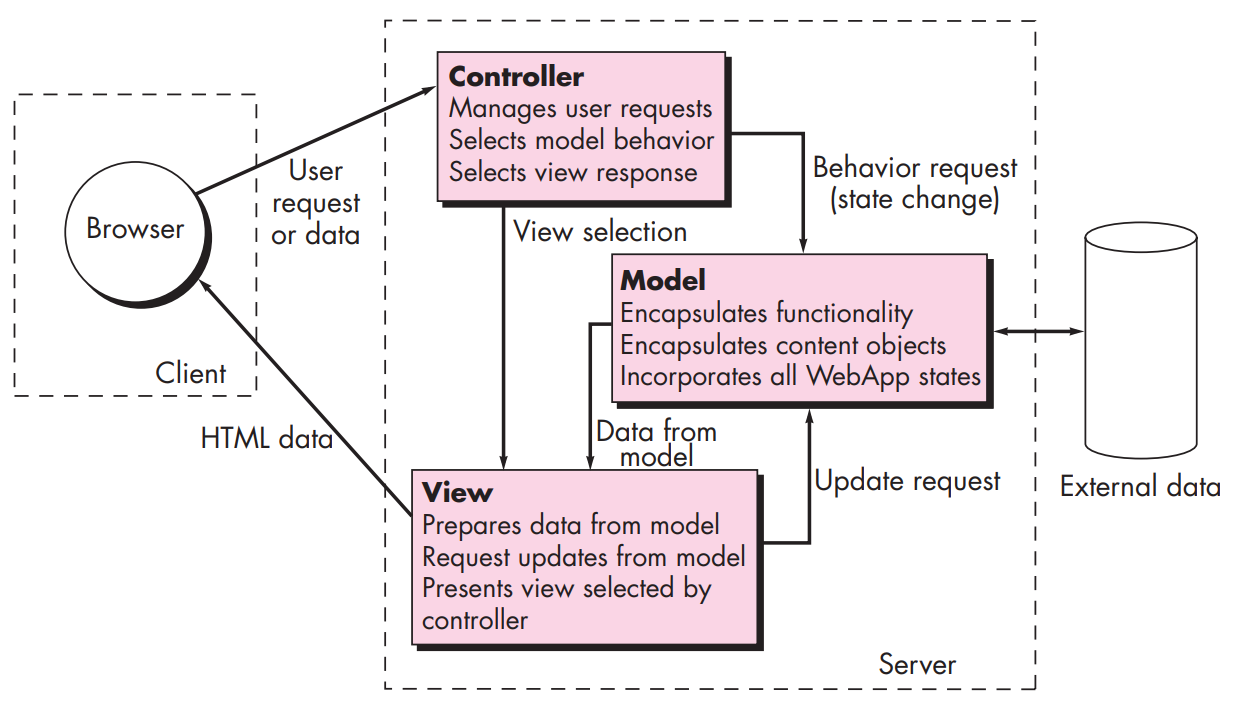
\includegraphics[width=0.68\textwidth]{arquitetura-mvc.png}
        \end{center}
    \label{dataMVCArchitecture}
    \legend{Fonte: \cite{pressman}}
\end{figure}

A arquitetura foi desenvolvida através, novamente, da linguagem de programação PHP. Para auxiliar na abstração e no desacoplamento entre os três módulos da arquitetura MVC, foi utilizado o motor de template Twig\footnote{\url{https://twig.symfony.com/} Acesso em outubro de 2018}. A ferramenta Twig  permite escrever um código mais conciso, com \textit{templates} mais legíveis e amigáveis para \textit{web designers} e, em vários casos, mais poderosos que \textit{templates} padrões do PHP \cite{symfonyBook}.

\begin{figure}[ht]
    \caption{Exemplo de \textit{template} padrão em PHP.}
       	\begin{center}
            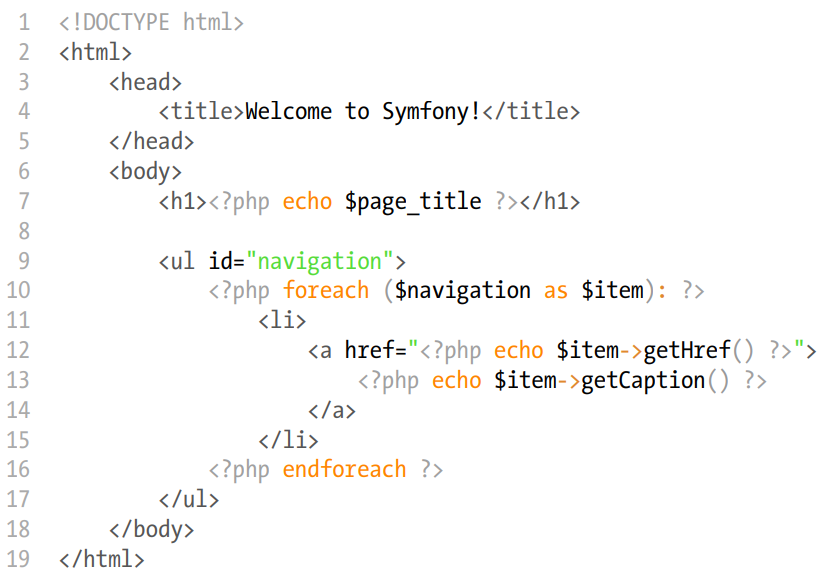
\includegraphics[width=0.68\textwidth]{twig-php.png}
        \end{center}
    \label{codeTemplatePHP}
    \legend{Fonte: \cite{symfonySensioLabs}}
\end{figure}

\bigskip

\begin{figure}[ht]
    \caption{Exemplo de \textit{template} em Twig .}
       	\begin{center}
            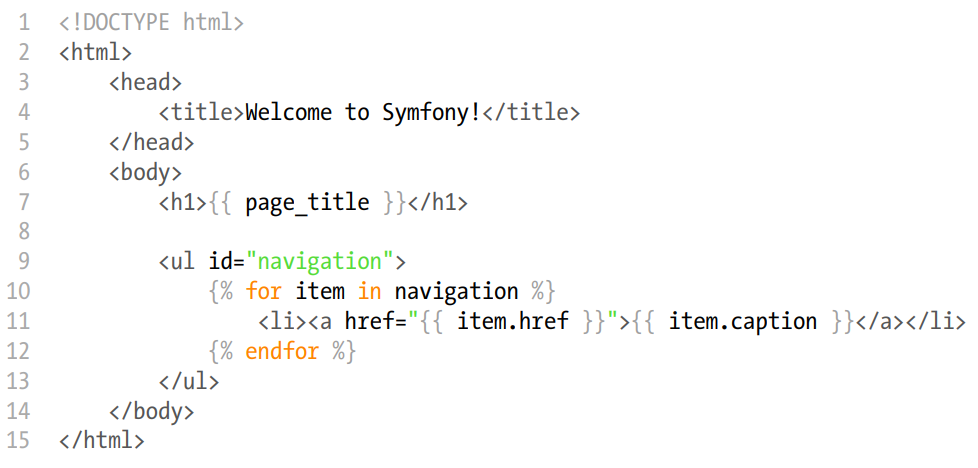
\includegraphics[width=0.68\textwidth]{figuras/twig-symf.png}
        \end{center}
    \label{codeTemplateTwig}
    \legend{Fonte: \cite{symfonySensioLabs}}
\end{figure}


\section{Projeto de Banco de dados}
\label{metodologiaBD}

\subsection{Modelagem dos dados}
\label{BDModelagem}

\subsection{Criação do banco de dados}
\label{BDCriacao}

\section{Implementação}
\label{metodologiaImplementação}

\subsection{Configuração do ambiente do trabalho}
\label{implementacaoConfig}

\subsection{SCRUM}
\label{implementacaoSCRUM}

\subsection{Versão inicial}
\label{implementacaoIR}

\subsection{Versão Alfa}
\label{implementacaoAR}

\subsection{Versão Beta}
\label{implementacaoBR}

\subsection{Versão Final}
\label{implementacaoFR}

% ========== CAP 4 ==============
\chapter{A rede social Portal de Vagas}
\label{redeSocialPortal}

% ========== CAP 5 ==============
\chapter{Avaliação com os usuários}
\label{Avaliação}

% ============== CAP 6 - CONCLUSÃO - =========================
\chapter{Conclusões}
\label{conclusao}




% ============== NÃO MEXER =========================
\bibliographystyle{abntex2-alf}
\bibliography{biblio}
% ============== NÃO MEXER =========================

\end{document}
